% Options for packages loaded elsewhere
\PassOptionsToPackage{unicode}{hyperref}
\PassOptionsToPackage{hyphens}{url}
%
\documentclass[
]{article}
\usepackage{lmodern}
\usepackage{amsmath}
\usepackage{ifxetex,ifluatex}
\ifnum 0\ifxetex 1\fi\ifluatex 1\fi=0 % if pdftex
  \usepackage[T1]{fontenc}
  \usepackage[utf8]{inputenc}
  \usepackage{textcomp} % provide euro and other symbols
  \usepackage{amssymb}
\else % if luatex or xetex
  \usepackage{unicode-math}
  \defaultfontfeatures{Scale=MatchLowercase}
  \defaultfontfeatures[\rmfamily]{Ligatures=TeX,Scale=1}
\fi
% Use upquote if available, for straight quotes in verbatim environments
\IfFileExists{upquote.sty}{\usepackage{upquote}}{}
\IfFileExists{microtype.sty}{% use microtype if available
  \usepackage[]{microtype}
  \UseMicrotypeSet[protrusion]{basicmath} % disable protrusion for tt fonts
}{}
\makeatletter
\@ifundefined{KOMAClassName}{% if non-KOMA class
  \IfFileExists{parskip.sty}{%
    \usepackage{parskip}
  }{% else
    \setlength{\parindent}{0pt}
    \setlength{\parskip}{6pt plus 2pt minus 1pt}}
}{% if KOMA class
  \KOMAoptions{parskip=half}}
\makeatother
\usepackage{xcolor}
\IfFileExists{xurl.sty}{\usepackage{xurl}}{} % add URL line breaks if available
\IfFileExists{bookmark.sty}{\usepackage{bookmark}}{\usepackage{hyperref}}
\hypersetup{
  pdftitle={Final Project},
  pdfauthor={Samruddhi Shinde},
  hidelinks,
  pdfcreator={LaTeX via pandoc}}
\urlstyle{same} % disable monospaced font for URLs
\usepackage[margin=1in]{geometry}
\usepackage{color}
\usepackage{fancyvrb}
\newcommand{\VerbBar}{|}
\newcommand{\VERB}{\Verb[commandchars=\\\{\}]}
\DefineVerbatimEnvironment{Highlighting}{Verbatim}{commandchars=\\\{\}}
% Add ',fontsize=\small' for more characters per line
\usepackage{framed}
\definecolor{shadecolor}{RGB}{248,248,248}
\newenvironment{Shaded}{\begin{snugshade}}{\end{snugshade}}
\newcommand{\AlertTok}[1]{\textcolor[rgb]{0.94,0.16,0.16}{#1}}
\newcommand{\AnnotationTok}[1]{\textcolor[rgb]{0.56,0.35,0.01}{\textbf{\textit{#1}}}}
\newcommand{\AttributeTok}[1]{\textcolor[rgb]{0.77,0.63,0.00}{#1}}
\newcommand{\BaseNTok}[1]{\textcolor[rgb]{0.00,0.00,0.81}{#1}}
\newcommand{\BuiltInTok}[1]{#1}
\newcommand{\CharTok}[1]{\textcolor[rgb]{0.31,0.60,0.02}{#1}}
\newcommand{\CommentTok}[1]{\textcolor[rgb]{0.56,0.35,0.01}{\textit{#1}}}
\newcommand{\CommentVarTok}[1]{\textcolor[rgb]{0.56,0.35,0.01}{\textbf{\textit{#1}}}}
\newcommand{\ConstantTok}[1]{\textcolor[rgb]{0.00,0.00,0.00}{#1}}
\newcommand{\ControlFlowTok}[1]{\textcolor[rgb]{0.13,0.29,0.53}{\textbf{#1}}}
\newcommand{\DataTypeTok}[1]{\textcolor[rgb]{0.13,0.29,0.53}{#1}}
\newcommand{\DecValTok}[1]{\textcolor[rgb]{0.00,0.00,0.81}{#1}}
\newcommand{\DocumentationTok}[1]{\textcolor[rgb]{0.56,0.35,0.01}{\textbf{\textit{#1}}}}
\newcommand{\ErrorTok}[1]{\textcolor[rgb]{0.64,0.00,0.00}{\textbf{#1}}}
\newcommand{\ExtensionTok}[1]{#1}
\newcommand{\FloatTok}[1]{\textcolor[rgb]{0.00,0.00,0.81}{#1}}
\newcommand{\FunctionTok}[1]{\textcolor[rgb]{0.00,0.00,0.00}{#1}}
\newcommand{\ImportTok}[1]{#1}
\newcommand{\InformationTok}[1]{\textcolor[rgb]{0.56,0.35,0.01}{\textbf{\textit{#1}}}}
\newcommand{\KeywordTok}[1]{\textcolor[rgb]{0.13,0.29,0.53}{\textbf{#1}}}
\newcommand{\NormalTok}[1]{#1}
\newcommand{\OperatorTok}[1]{\textcolor[rgb]{0.81,0.36,0.00}{\textbf{#1}}}
\newcommand{\OtherTok}[1]{\textcolor[rgb]{0.56,0.35,0.01}{#1}}
\newcommand{\PreprocessorTok}[1]{\textcolor[rgb]{0.56,0.35,0.01}{\textit{#1}}}
\newcommand{\RegionMarkerTok}[1]{#1}
\newcommand{\SpecialCharTok}[1]{\textcolor[rgb]{0.00,0.00,0.00}{#1}}
\newcommand{\SpecialStringTok}[1]{\textcolor[rgb]{0.31,0.60,0.02}{#1}}
\newcommand{\StringTok}[1]{\textcolor[rgb]{0.31,0.60,0.02}{#1}}
\newcommand{\VariableTok}[1]{\textcolor[rgb]{0.00,0.00,0.00}{#1}}
\newcommand{\VerbatimStringTok}[1]{\textcolor[rgb]{0.31,0.60,0.02}{#1}}
\newcommand{\WarningTok}[1]{\textcolor[rgb]{0.56,0.35,0.01}{\textbf{\textit{#1}}}}
\usepackage{graphicx}
\makeatletter
\def\maxwidth{\ifdim\Gin@nat@width>\linewidth\linewidth\else\Gin@nat@width\fi}
\def\maxheight{\ifdim\Gin@nat@height>\textheight\textheight\else\Gin@nat@height\fi}
\makeatother
% Scale images if necessary, so that they will not overflow the page
% margins by default, and it is still possible to overwrite the defaults
% using explicit options in \includegraphics[width, height, ...]{}
\setkeys{Gin}{width=\maxwidth,height=\maxheight,keepaspectratio}
% Set default figure placement to htbp
\makeatletter
\def\fps@figure{htbp}
\makeatother
\setlength{\emergencystretch}{3em} % prevent overfull lines
\providecommand{\tightlist}{%
  \setlength{\itemsep}{0pt}\setlength{\parskip}{0pt}}
\setcounter{secnumdepth}{-\maxdimen} % remove section numbering
\ifluatex
  \usepackage{selnolig}  % disable illegal ligatures
\fi

\title{Final Project}
\author{Samruddhi Shinde}
\date{5/1/2021}

\begin{document}
\maketitle

Loading packages

\begin{Shaded}
\begin{Highlighting}[]
\FunctionTok{library}\NormalTok{(here)}
\end{Highlighting}
\end{Shaded}

\begin{verbatim}
## here() starts at /Users/SammyShinde/Desktop/GitHub/hw-samruddhis/final_project
\end{verbatim}

\begin{Shaded}
\begin{Highlighting}[]
\FunctionTok{library}\NormalTok{(tidyverse)}
\end{Highlighting}
\end{Shaded}

\begin{verbatim}
## -- Attaching packages --------------------------------------- tidyverse 1.3.0 --
\end{verbatim}

\begin{verbatim}
## v ggplot2 3.3.3     v purrr   0.3.4
## v tibble  3.0.6     v dplyr   1.0.3
## v tidyr   1.1.2     v stringr 1.4.0
## v readr   1.4.0     v forcats 0.5.1
\end{verbatim}

\begin{verbatim}
## -- Conflicts ------------------------------------------ tidyverse_conflicts() --
## x dplyr::filter() masks stats::filter()
## x dplyr::lag()    masks stats::lag()
\end{verbatim}

Loading in Dataset

\begin{Shaded}
\begin{Highlighting}[]
\NormalTok{covid\_prison\_cases }\OtherTok{\textless{}{-}} \FunctionTok{read\_csv}\NormalTok{(}\FunctionTok{here}\NormalTok{(}\StringTok{"data"}\NormalTok{, }\StringTok{"covid\_prison\_cases.csv"}\NormalTok{))}
\end{Highlighting}
\end{Shaded}

\begin{verbatim}
## 
## -- Column specification --------------------------------------------------------
## cols(
##   name = col_character(),
##   abbreviation = col_character(),
##   staff_tests = col_double(),
##   staff_tests_with_multiples = col_double(),
##   total_staff_cases = col_double(),
##   staff_recovered = col_double(),
##   total_staff_deaths = col_double(),
##   prisoner_tests = col_double(),
##   prisoner_tests_with_multiples = col_double(),
##   total_prisoner_cases = col_double(),
##   prisoners_recovered = col_double(),
##   total_prisoner_deaths = col_double(),
##   as_of_date = col_character(),
##   notes = col_character()
## )
\end{verbatim}

This dataset explores COVID-19 data in prisons across the United States.

Data Set of Covid-19 Cases for every State in March 2021

\begin{Shaded}
\begin{Highlighting}[]
\NormalTok{march2021\_covid\_cases }\OtherTok{\textless{}{-}}\NormalTok{ covid\_prison\_cases }\SpecialCharTok{\%\textgreater{}\%}
  \FunctionTok{filter}\NormalTok{(as\_of\_date }\SpecialCharTok{==} \StringTok{"03/01/2021"}\SpecialCharTok{|} 
\NormalTok{        as\_of\_date }\SpecialCharTok{==}\StringTok{"03/02/2021"}\SpecialCharTok{|} 
\NormalTok{        as\_of\_date }\SpecialCharTok{==}\StringTok{"03/03/2021"}\SpecialCharTok{|} 
\NormalTok{        as\_of\_date }\SpecialCharTok{==} \StringTok{"03/04/2021"}\SpecialCharTok{|} 
\NormalTok{        as\_of\_date }\SpecialCharTok{==}\StringTok{"03/05/2021"}\NormalTok{) }
\end{Highlighting}
\end{Shaded}

Bar plot Covid-19 Cases for every State in March 2021

\begin{Shaded}
\begin{Highlighting}[]
\NormalTok{march2021\_covid\_cases }\SpecialCharTok{\%\textgreater{}\%}
  \FunctionTok{ggplot}\NormalTok{(aes}
\NormalTok{         (}\AttributeTok{x =}\NormalTok{ abbreviation, }
          \AttributeTok{y =}\NormalTok{ total\_prisoner\_cases,}
          \AttributeTok{color =}\NormalTok{ abbreviation,}
           \AttributeTok{fill =}\NormalTok{ abbreviation)) }\SpecialCharTok{+}
  \FunctionTok{geom\_bar}\NormalTok{(}\AttributeTok{stat=}\StringTok{"identity"}\NormalTok{, }\AttributeTok{alpha=}\NormalTok{.}\DecValTok{8}\NormalTok{, }\AttributeTok{width=}\NormalTok{.}\DecValTok{6}\NormalTok{) }\SpecialCharTok{+}
  \FunctionTok{theme}\NormalTok{(}\AttributeTok{axis.text.x  =} \FunctionTok{element\_text}\NormalTok{(}\AttributeTok{angle=}\SpecialCharTok{{-}}\DecValTok{90}\NormalTok{, }\AttributeTok{hjust=}\FloatTok{0.5}\NormalTok{, }\AttributeTok{size=}\DecValTok{7}\NormalTok{,}\AttributeTok{colour=}\StringTok{"black"}\NormalTok{)) }\SpecialCharTok{+}
  \FunctionTok{ggtitle}\NormalTok{(}\StringTok{"COVID{-}19 Cases in US Prisoners in March 2021"}\NormalTok{) }\SpecialCharTok{+}
  \FunctionTok{ylab}\NormalTok{(}\StringTok{"Number of Cases"}\NormalTok{) }\SpecialCharTok{+}
  \FunctionTok{xlab}\NormalTok{(}\StringTok{"State"}\NormalTok{) }\SpecialCharTok{+}
  \FunctionTok{theme}\NormalTok{(}\AttributeTok{legend.title =} \FunctionTok{element\_blank}\NormalTok{())}
\end{Highlighting}
\end{Shaded}

\begin{verbatim}
## Warning: Removed 1 rows containing missing values (position_stack).
\end{verbatim}

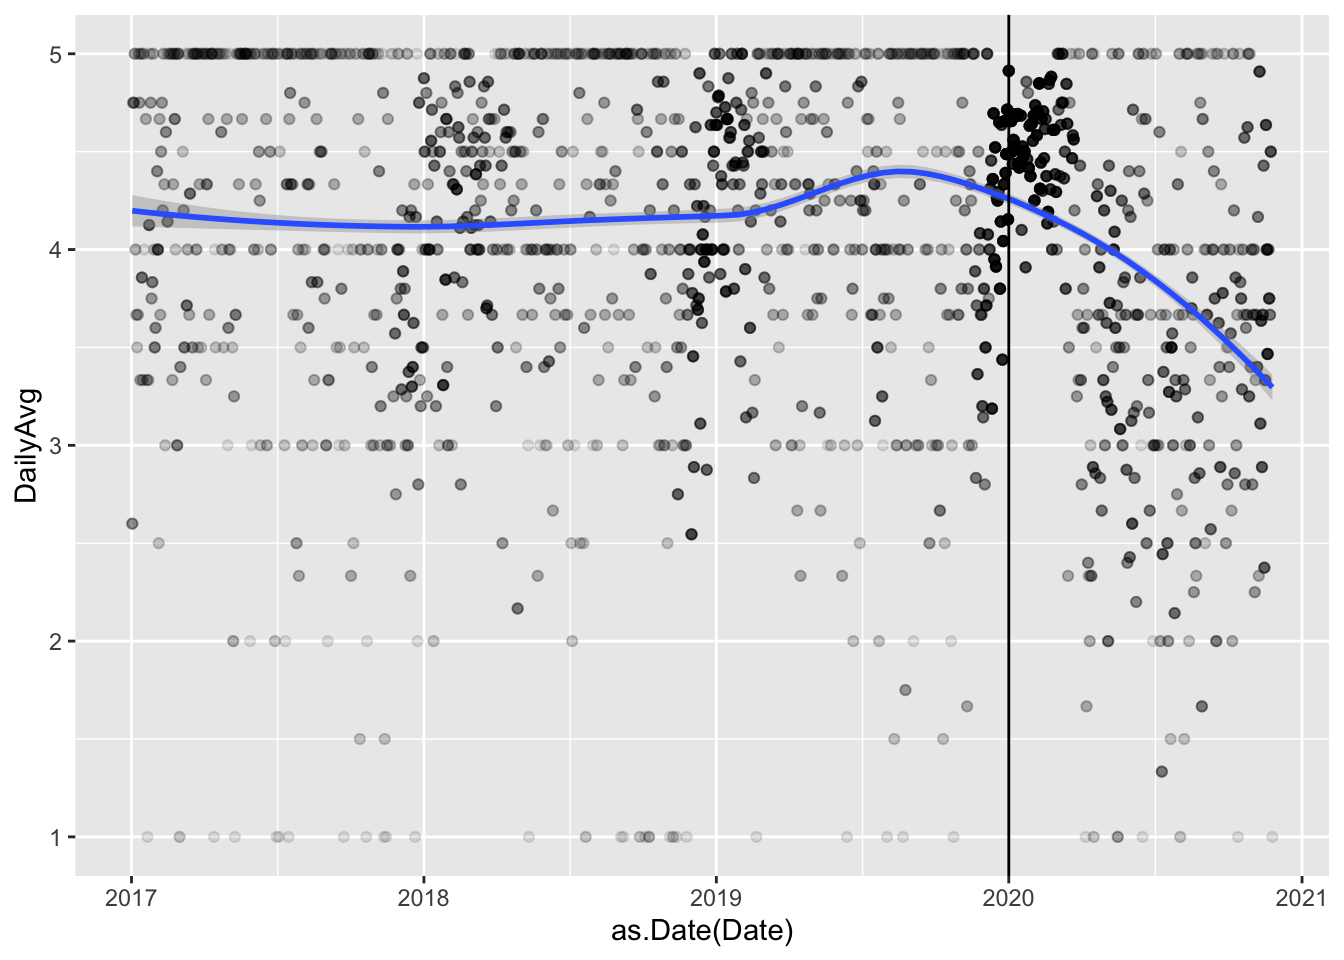
\includegraphics{final_project_files/figure-latex/unnamed-chunk-4-1.pdf}
This bar graph shows that California and federal prisons had the highest
cases of COVID-19 in prisoners in March 2021.

\begin{Shaded}
\begin{Highlighting}[]
\NormalTok{us\_covid\_stats }\OtherTok{\textless{}{-}}\NormalTok{ march2021\_covid\_cases }\SpecialCharTok{\%\textgreater{}\%}
  \FunctionTok{summarize}\NormalTok{(}\AttributeTok{Average\_Staff\_Cases =} \FunctionTok{mean}\NormalTok{(total\_staff\_cases, }\AttributeTok{na.rm =} \ConstantTok{TRUE}\NormalTok{),}
            \AttributeTok{Min\_Staff\_Cases =} \FunctionTok{min}\NormalTok{(total\_staff\_cases, }\AttributeTok{na.rm =} \ConstantTok{TRUE}\NormalTok{),}
            \AttributeTok{Max\_Staff\_Cases =} \FunctionTok{max}\NormalTok{(total\_staff\_cases, }\AttributeTok{na.rm =} \ConstantTok{TRUE}\NormalTok{),}
            \AttributeTok{Average\_Staff\_Deaths =} \FunctionTok{mean}\NormalTok{(total\_staff\_deaths, }\AttributeTok{na.rm =} \ConstantTok{TRUE}\NormalTok{),}
            \AttributeTok{Min\_Staff\_Deaths =} \FunctionTok{min}\NormalTok{(total\_staff\_deaths, }\AttributeTok{na.rm =} \ConstantTok{TRUE}\NormalTok{),}
            \AttributeTok{Max\_Staff\_Deaths =} \FunctionTok{max}\NormalTok{(total\_staff\_deaths, }\AttributeTok{na.rm =} \ConstantTok{TRUE}\NormalTok{),}
            \AttributeTok{Average\_Prisoner\_Cases =} \FunctionTok{mean}\NormalTok{(total\_prisoner\_cases, }\AttributeTok{na.rm =} \ConstantTok{TRUE}\NormalTok{),}
            \AttributeTok{Min\_Prisoner\_Cases =} \FunctionTok{min}\NormalTok{(total\_prisoner\_cases, }\AttributeTok{na.rm =} \ConstantTok{TRUE}\NormalTok{),}
            \AttributeTok{Maz\_Prisoner\_Cases =} \FunctionTok{max}\NormalTok{(total\_prisoner\_cases, }\AttributeTok{na.rm =} \ConstantTok{TRUE}\NormalTok{),}
            \AttributeTok{Average\_Prisoner\_Deaths =} \FunctionTok{mean}\NormalTok{(total\_prisoner\_deaths, }\AttributeTok{na.rm =} \ConstantTok{TRUE}\NormalTok{),}
            \AttributeTok{Min\_Prisoner\_Deaths =} \FunctionTok{min}\NormalTok{(total\_prisoner\_deaths, }\AttributeTok{na.rm =} \ConstantTok{TRUE}\NormalTok{),}
            \AttributeTok{Max\_Prisoner\_Deaths =} \FunctionTok{max}\NormalTok{(total\_prisoner\_deaths, }\AttributeTok{na.rm =} \ConstantTok{TRUE}\NormalTok{))}

\FunctionTok{tibble}\NormalTok{(us\_covid\_stats)}
\end{Highlighting}
\end{Shaded}

\begin{verbatim}
## # A tibble: 1 x 12
##   Average_Staff_C~ Min_Staff_Cases Max_Staff_Cases Average_Staff_D~
##              <dbl>           <dbl>           <dbl>            <dbl>
## 1            2217.              57           15810             4.75
## # ... with 8 more variables: Min_Staff_Deaths <dbl>, Max_Staff_Deaths <dbl>,
## #   Average_Prisoner_Cases <dbl>, Min_Prisoner_Cases <dbl>,
## #   Maz_Prisoner_Cases <dbl>, Average_Prisoner_Deaths <dbl>,
## #   Min_Prisoner_Deaths <dbl>, Max_Prisoner_Deaths <dbl>
\end{verbatim}

This table shows that on average, prisoners have higher case \& death
rates compared to staff.

Filtering the covid\_prison\_cases dataset for California statistics
Also only looking at staff \& prisoner cases/deaths

\begin{Shaded}
\begin{Highlighting}[]
\NormalTok{cali\_covid\_cases }\OtherTok{\textless{}{-}}\NormalTok{ covid\_prison\_cases }\SpecialCharTok{\%\textgreater{}\%}
  \FunctionTok{filter}\NormalTok{(name }\SpecialCharTok{==} \StringTok{"California"}\NormalTok{) }\SpecialCharTok{\%\textgreater{}\%}
  \FunctionTok{select}\NormalTok{(total\_staff\_cases, total\_staff\_deaths, total\_prisoner\_cases, total\_prisoner\_deaths, as\_of\_date)}
\end{Highlighting}
\end{Shaded}

Summary table of average \& sd of staff cases/deaths and prisoner
cases/deaths

\begin{Shaded}
\begin{Highlighting}[]
\NormalTok{cali\_covid\_stats }\OtherTok{\textless{}{-}}\NormalTok{ cali\_covid\_cases }\SpecialCharTok{\%\textgreater{}\%}
  \FunctionTok{summarize}\NormalTok{(}\AttributeTok{Average\_Staff\_Cases =} \FunctionTok{mean}\NormalTok{(total\_staff\_cases, }\AttributeTok{na.rm =} \ConstantTok{TRUE}\NormalTok{),}
            \AttributeTok{Min\_Staff\_Cases =} \FunctionTok{min}\NormalTok{(total\_staff\_cases, }\AttributeTok{na.rm =} \ConstantTok{TRUE}\NormalTok{),}
            \AttributeTok{Max\_Staff\_Cases =} \FunctionTok{max}\NormalTok{(total\_staff\_cases, }\AttributeTok{na.rm =} \ConstantTok{TRUE}\NormalTok{),}
            \AttributeTok{Average\_Staff\_Deaths =} \FunctionTok{mean}\NormalTok{(total\_staff\_deaths, }\AttributeTok{na.rm =} \ConstantTok{TRUE}\NormalTok{),}
            \AttributeTok{Min\_Staff\_Deaths =} \FunctionTok{min}\NormalTok{(total\_staff\_deaths, }\AttributeTok{na.rm =} \ConstantTok{TRUE}\NormalTok{),}
            \AttributeTok{Max\_Staff\_Deaths =} \FunctionTok{max}\NormalTok{(total\_staff\_deaths, }\AttributeTok{na.rm =} \ConstantTok{TRUE}\NormalTok{),}
            \AttributeTok{Average\_Prisoner\_Cases =} \FunctionTok{mean}\NormalTok{(total\_prisoner\_cases, }\AttributeTok{na.rm =} \ConstantTok{TRUE}\NormalTok{),}
            \AttributeTok{Min\_Prisoner\_Cases =} \FunctionTok{min}\NormalTok{(total\_prisoner\_cases, }\AttributeTok{na.rm =} \ConstantTok{TRUE}\NormalTok{),}
            \AttributeTok{Maz\_Prisoner\_Cases =} \FunctionTok{max}\NormalTok{(total\_prisoner\_cases, }\AttributeTok{na.rm =} \ConstantTok{TRUE}\NormalTok{),}
            \AttributeTok{Average\_Prisoner\_Deaths =} \FunctionTok{mean}\NormalTok{(total\_prisoner\_deaths, }\AttributeTok{na.rm =} \ConstantTok{TRUE}\NormalTok{),}
            \AttributeTok{Min\_Prisoner\_Deaths =} \FunctionTok{min}\NormalTok{(total\_prisoner\_deaths, }\AttributeTok{na.rm =} \ConstantTok{TRUE}\NormalTok{),}
            \AttributeTok{Max\_Prisoner\_Deaths =} \FunctionTok{max}\NormalTok{(total\_prisoner\_deaths, }\AttributeTok{na.rm =} \ConstantTok{TRUE}\NormalTok{))}

\FunctionTok{tibble}\NormalTok{(cali\_covid\_stats)}
\end{Highlighting}
\end{Shaded}

\begin{verbatim}
## # A tibble: 1 x 12
##   Average_Staff_C~ Min_Staff_Cases Max_Staff_Cases Average_Staff_D~
##              <dbl>           <dbl>           <dbl>            <dbl>
## 1            5035.               9           15810             8.41
## # ... with 8 more variables: Min_Staff_Deaths <dbl>, Max_Staff_Deaths <dbl>,
## #   Average_Prisoner_Cases <dbl>, Min_Prisoner_Cases <dbl>,
## #   Maz_Prisoner_Cases <dbl>, Average_Prisoner_Deaths <dbl>,
## #   Min_Prisoner_Deaths <dbl>, Max_Prisoner_Deaths <dbl>
\end{verbatim}

This table shows that on average, prisoners in California have higher
case \& death rates compared to staff.

Filtering data to only look at 2020 cases

\begin{Shaded}
\begin{Highlighting}[]
\NormalTok{cali\_2020covid\_cases }\OtherTok{\textless{}{-}}\NormalTok{ cali\_covid\_cases[}\SpecialCharTok{{-}}\FunctionTok{c}\NormalTok{(}\DecValTok{1}\SpecialCharTok{:}\DecValTok{9}\NormalTok{),]}
\end{Highlighting}
\end{Shaded}

Scatter Plot for total prisoner cases per date

\begin{Shaded}
\begin{Highlighting}[]
\NormalTok{cali\_2020covid\_cases }\SpecialCharTok{\%\textgreater{}\%}
  \FunctionTok{ggplot}\NormalTok{(aes}
\NormalTok{         (}\AttributeTok{x =}\NormalTok{ as\_of\_date,}
           \AttributeTok{y =}\NormalTok{ total\_prisoner\_cases)) }\SpecialCharTok{+}
  \FunctionTok{geom\_point}\NormalTok{() }\SpecialCharTok{+}
  \FunctionTok{theme}\NormalTok{(}\AttributeTok{axis.text.x =} \FunctionTok{element\_text}\NormalTok{(}\AttributeTok{angle =} \DecValTok{90}\NormalTok{, }\AttributeTok{vjust =} \FloatTok{0.5}\NormalTok{, }\AttributeTok{hjust=}\DecValTok{1}\NormalTok{)) }\SpecialCharTok{+}
  \FunctionTok{ggtitle}\NormalTok{(}\StringTok{"COVID{-}19 Cases in Califronia Prisoners in 2020"}\NormalTok{) }\SpecialCharTok{+}
  \FunctionTok{ylab}\NormalTok{(}\StringTok{"Total Number of Cases"}\NormalTok{) }\SpecialCharTok{+}
  \FunctionTok{xlab}\NormalTok{(}\StringTok{"Date"}\NormalTok{) }
\end{Highlighting}
\end{Shaded}

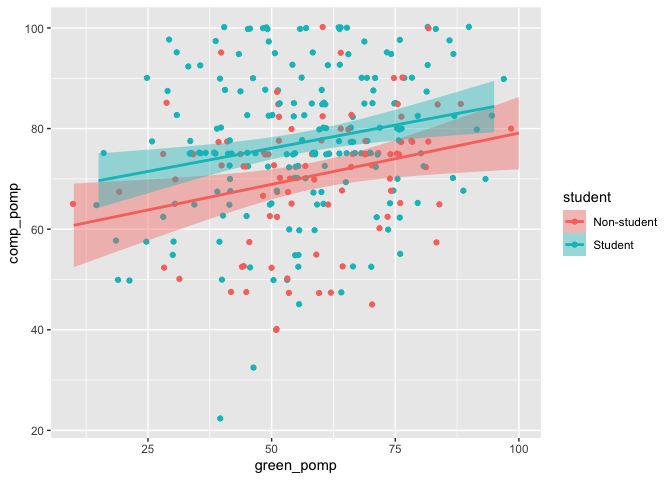
\includegraphics{final_project_files/figure-latex/unnamed-chunk-9-1.pdf}

This scatter plot shows the trend of increasing COVID-19 cases in
prisoners during 2020.

\end{document}
